\chapter{Methods}

The aim of the methods described in this thesis is to develop and characterise tools that elucidate the status of mutation disequilibrium in DNA sequences. In this chapter I present a test of disequilibrium existence (Section \ref{Test of Existence}) and tests of equivalence between evolutionary processes (Section \ref{Tests of Equivalence of Process}). Additionally, I present two novel statistics for measuring the magnitude of disequilibrium (Sections \ref{nabla} and \ref{T50}). 

\section{Data Sets}

\subsubsection{Microbial}

To establish the properties of my methods on alignments of taxa that range in their evolutionary divergence, I chose a widely used molecular marker of microbial genetic diversity. Hereafter, I will refer to this data as the Microbial data. The Microbial data is a subset of GreneGenes, a database of curated alignments of 16S ribosomal RNA (rRNA) sequences \citep{McDonald2012AnArchaea}. The sequences were aligned using an alignment algorithm that uses knowledge of rRNA secondary structure and conserved residues \citep{McDonald2012AnArchaea}. The Microbial data consists of 9,702 alignments of species triples that were sampled from GreneGenes with an approximately uniform representation of maximum Jensen-Shannon Divergence (JSD). Details of the sampling process are described in \citep{Kaehler2015}. An important side effect of the sampling process is that a species can appear in more than one triple, so not each alignment is independent. The Microbial data was downloaded from Dryad (\href{https://doi.org/10.5061/dryad.g7g0n}{https://doi.org/10.5061/dryad.g7g0n}).  

\subsubsection{Drosophila}

In order to test for elevated mutation disequilibrium in \textit{D. melanogaster}, I sampled protein coding sequence (CDS) alignments of one-to-one orthologs from \textit{D. melanogaster}, \textit{D. simulans} and \textit{Drosophila yakubra}. Hereafter, the \textit{Drosophila} data, this contains 9237 alignments of one-to-one orthologs of CDS obtained from \textit{flyDIVaS}, a database of curated \textit{D. melanogaster}-centric orthologous gene sets \citep{Stanley2016FlyDIVaS:Selection, Clark2007EvolutionPhylogeny}. The \textit{flyDIVaS} pipeline extracts protein-coding genes from the latest FlyBase release, identifying one-to-one orthologs using OrthoDB \citep{Zdobnov2021OrthoDBOrthologs}. The alignments were provided by \textit{flyDIVaS}, the pipeline used first aligns protein sequences using MUSCLE \citep{Edgar2004MUSCLE:Complexity}, before the alignments were backtranslated to CDS, filtered and masked. Further details of the sampling and alignment process are described in \citep{Stanley2016FlyDIVaS:Selection}. 

\subsubsection{Rodent}

To establish the impact of translocation to the PAR on the \textit{Fxy} gene in \textit{M. musculus}, I sampled one-to-one orthologs of \textit{Fxy} from \textit{M. spretus} and \textit{Rattus norvegicus}, in which \textit{Fxy} is X-linked. Intronic \textit{Fxy} sequences for all species were sampled using EnsemblDb3, an open-source python tool for querying Ensembl for related sequences \citep{HuttleyEnsembldb3}. The first eight introns of \textit{Fxy} were aligned using the Cogent3 progressive nucleotide aligner with default settings \citep{Knight2007PyCogent:Sequence}. The model used for alignment was HKY85 \citep{Hasegawa1985DatingDNA}, all parameters were saved in a log file for which the indel length=0.1, indel rate=1e-10, $\kappa=3$. 

\subsubsection{Great Apes}

Sampling CDS and introns from the same gene enables paired comparison of the two sequence types. The human genome, as well as those for many of the great apes, are an extremely well-curated genomic resource. Ensembl Compara contains annotated genome-wide species comparison data where annotation of orthology is quality controlled using synteny \citep{Herrero2016EnsemblResources}. Data for the Great Apes intronic and CDS data sets were sampled from Ensembl release 104 \citep{Howe2021Ensembl2021}. From \textit{Homo sapiens} (human) protein coding genes of chromosome 1 I identified one-to-one orthologs in \textit{Pan troglodytes} (chimpanzee) and \textit{Gorilla gorilla} (gorilla) using EnsemblDb3 \citep{HuttleyEnsembldb3} and homologsampler \citep{HuttleyHomologsampler}, open-source python tools for querying Ensembl for related sequences. From this gene list I sampled the CDS from the canonical transcript of unaligned one-to-one orthologs \cite{Howe2021Ensembl2021}. To sample the introns, all exons were filtered resulting in an alignment of concatenated introns. The introns were aligned by Ensembl using the EPO alignment pipeline (the method link id was 1944) \citep{Howe2021Ensembl2021}. I aligned CDS using the Cogent3 progressive codon aligner \citep{Knight2007PyCogent:Sequence}. The codon model was MG94HKY \citep{Muse1994AGenome}, the codon parameters were: indel length=0.1; indel rate=1e-10; $\omega=0.4; \kappa=3$. 

\subsection{Data Filtering}
\label{Data Filtering}

Substitution models are explicitly restricted to interchanges between nucleotide states, so alignment positions linked to other mutation types were removed. This includes gap characters, representing an insertion-deletion event, and annotated simple tandem repeats, likely to have evolved through strand slippage \citep{Levinson1987Slipped-strandEvolution}. For all CDS, to reduce the impact of selection, I filtered to include sites corresponding to the third codon position only. Alignments shorter than $300$bp after filtering were excluded. Summary statistics of the raw and filtered alignments are shown in Table \ref{tab:seq_summary}. 

\begin{table}[ht]
\centering
\small
\setstretch{1.4}
\begin{tabularx}{\textwidth}{ 
  | >{\centering\arraybackslash}c
  | >{\arraybackslash}X 
  | >{\centering\arraybackslash}X 
  | >{\centering\arraybackslash}X 
  | >{\centering\arraybackslash}X 
  | >{\centering\arraybackslash}X | }
\hline
&  & \multicolumn{2}{c |}{\textbf{Raw}} & \multicolumn{2}{c |}{\textbf{Filtered}} \\ 
\hline
\textbf{Data Set} & Taxa & Number of Alignments & Min, Median, and Max Sequence Length (bp) & Number of Alignments & Min, Median, and Max Sequence Length (bp) \\

\hline

Microbial & * & - & - & 9,854 & 924, 1,138, 1,276  \\

\hline

Drosophila  & \hbox{\textbf{\textit{D. melanogaster},}} \hbox{\textbf{\textit{D. simulans},}} \textit{D. yakubra} & 9,237 & 120, 1,287, 26,952 & 5,944 & 300, 1,230, 26,676  \\

\hline

Rodent & \hbox{\textbf{\textit{M. musculus}},} \hbox{\textbf{\textit{M. spretus},}} \hbox{\textit{R. norvegicus}} & 8 & 4,948, 26,680.5, 57,007 & 8 & 834, 7,062, 42,742 \\ 

\hline

\shortstack{ \\ Great Ape \\ Introns} & \textbf{Human}, \textbf{Chimp}, Gorilla & 1,481 & 103, 9,679, 298,974 & 1,406 & 302, 7,723.5, $274,635$ \\

\hline

\shortstack{ \\ Great Ape \\ CDS} & \textbf{Human}, \textbf{Chimp}, Gorilla & 1,683 & 165, 1,365, 26,775 & 1,182 & 300, 545.5, 8,601 \\

\hline

\end{tabularx}
\caption{\textbf{Summary of Data Sets.} The ingroup edges for each set of taxa are bolded. \\ \textbf{*} The Microbial data set is comprised of alignments of the same sequence, but for different triads of taxa. }
\label{tab:seq_summary}
\end{table}


I illustrate the impact of the filtering process using dotplots. A dotplot displays the relatedness of biological sequences showing matches as lines on the chart \citep{Gibbs1970TheSequences}. A randomly selected alignment from both the CDS and Intronic Great Ape data sets are shown in Figure \ref{fig:dotplots}. For both alignments, the plot on the left is pre-filtering, and the plot on the right is post-filtering. The $x$ and $y$ axes correspond to the indicated sequence. The dotted line is the coordinates of the alignment path. Long stretches of identity between the sequences form a diagonal. Matches of the forward strand are shown in blue, matches of the reverse complement are shown in red. Validation of the alignment methods is given by the alignment path sitting on top of the visual diagonal (Figure \ref{fig:dotplots}). Long stretches of tandem repeats show up as large blocks of colour, visible in the unfiltered intronic dotplot, Figure \ref{fig:dotplots}a. Figure \ref{fig:dotplots}b shows the same alignment, but after the filtering process, in which these repeated sequences have been removed.

\begin{figure}[htbp]
\centering
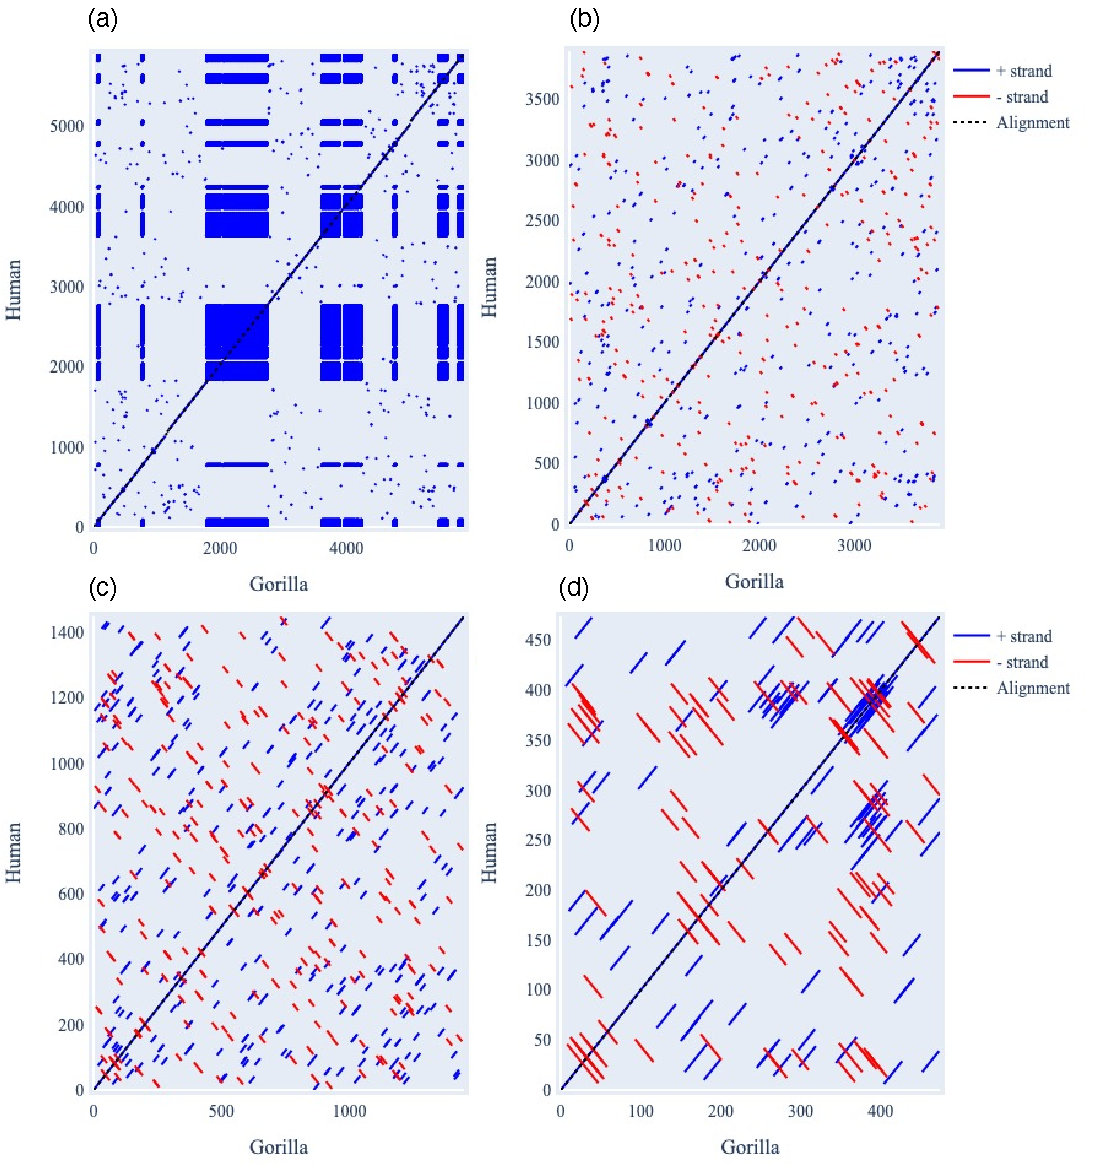
\includegraphics[width=\textwidth]{figures/diagrams/primate_dotplots.pdf}
\caption{Dotplots. Window was 20bp long, a match was considered if $>13$bp of the window of 20 were identical. }
\label{fig:dotplots}
\end{figure}

\section{Models}

Phylogenetics! the concept of a tree. Because all sampling was done in triple I assume an unrooted phylogeny. 

Substitution models describe the evolutionary process along the edge of a tree by modelling substitutions as a Markov process. For a nucleotide process, the possible states are the finite set of nucleotide bases $X = [A, C, G, T]$ and the state frequencies at the common ancestor is denoted $\pi$. Most commonly used are continuous-time processes, defined by a rate matrix denoted $\mathrm{Q}$. The elements of $\mathrm{Q}$ represent the instantaneous rate of change from the row label state (e.g. $A$) to a column label state (e.g. $T$). A discrete-time process is defined in terms of substitution probability matrix, denoted $\mathrm{P}$, in which elements represent the probabilities of substituting the row label state with the column label state in some time $t$ interval. For a continuous-time model, the two representations are related by the following, $\mathrm{P}(t) = e^{\mathrm{Q}t}$. 

In this work, I use three continuous-time models and one discrete-time model. General Nucleotide (GN) is a non-stationary and non-reversible nucleotide model for which time-homogeneity between nodes in the tree is the only required constraint \citep{Kaehler2015}. Using this model of evolution, there are 12 distinct rates taking place at any given site. General Nucleotide Stationary (GNS) is a general nucleotide Markov process that only differs from GN by its constraint of stationarity. That is, the base frequencies, do not change through time. The formulation of GNS is provided by Von Bing Yap and Gavin Huttley (Personal Communication). General Time Reversible (GTR) is a general nucleotide model that is constrained to be time-reversible and thus stationary \citep{Lanave1984ARates} and is a popular model of choice in the field. The Barry and Hartigan (BH) model is a general discrete-time Markov process for nucleotides \citep{Barry1987StatisticalEvolution}. The key assumptions for each model can be found in table \ref{model_assumptions}.

\begin{table}[htbp]
\centering
\begin{tabularx}{0.7\textwidth}{ 
  | >{\centering\arraybackslash}c 
  | >{\centering\arraybackslash}X 
  | >{\centering\arraybackslash}X  
  | >{\centering\arraybackslash}X | }
\hline  
\textbf{Assumption} & \textbf{BH} & \textbf{GN} & \textbf{GS}  \\
\hline 
    Reversibility & - & - & -  \\
    Stationarity & - & - & \checkmark  \\
    Time-Homogeneity  & - & \checkmark & \checkmark \\
    Independent sites & \checkmark & \checkmark & \checkmark\\ 
\hline 
\end{tabularx}
\caption{Markov process assumptions}
\label{model_assumptions}

\end{table}


For a continuous-time process, a genetic distance can be given in terms of the expected number of substitutions per site in a given time interval. For a non-stationary process, this requires a generalised measure \citep{Kaehler2015}. When applied to data satisfying the assumption of stationarity, this measure reduces to the standard formulation of genetic distance. As per \cite{Kaehler2015}, I denote this distance ENS. 


\subsection{Maximum Likelihood}

Maximum Likelihood (ML) is a well-established framework for statistical inference using substitution models. Under mild conditions ML is consistent, meaning that as the amount of data (the length of the alignment) tends to infinity, the probability of obtaining the true value of the parameters tends to one \citep{Chang1996FullConsistency}. A condition of proof is that the alignment contains at least three sequences \citep{Chang1996FullConsistency}, for that reason all data sampling created ensured three sequences. Given some data, the likelihood of a hypothesis is the probability of the data given that hypothesis. For likelihoods involving substitution models, the tree topology and the values of free parameters is the hypothesis. ML methods `fit' a model by returning the model parameters that produce the highest probability of generating the observed sequence data \citep{Felsenstein1981EvolutionaryApproach}.

ML is a powerful framework for determining whether there is significant improvement between \gls{nested} models. One `null' model is considered nested in another if it can be specified simply by imposing restrictions on the parameters of the `alternate' model.  For the models of interest, GNS is nested within GN as it can be specified by imposing the constraint of stationarity. For nested models, it is theoretically guaranteed that the likelihood for the alternate will be greater or equal to that for the null. 

A likelihood ratio test (LRT) is a method of comparing nested models. The LRT process is described in Figure \ref{fig:lrt}. An LRT is a test of whether additional components unique to the alternate model cause a significant improvement in the description of the data. Practically, this involves comparing likelihoods between models. The log-likelihood ($\ln\mathcal{L}$) for each model is obtained via fitting. The likelihood ratio (LR), is the ratio of the $\ln\mathcal{L}$ of the two models:
$$\mathrm{LR} = 2(\ln \mathcal{L}_{alt} -  \ln \mathcal{L}_{null}).$$
If the null model is appropriate and the length of the alignment is adequate, the LRT statistic will be $\chi^2_{df}$ distributed with degrees freedom (df) equal to the difference in the number of free parameters between the models \citep{Lindgren1993StatisticalTheory, Silvey1975StatisticalInference, Kendall1979The2}.

\begin{figure}[htbp]
\centering
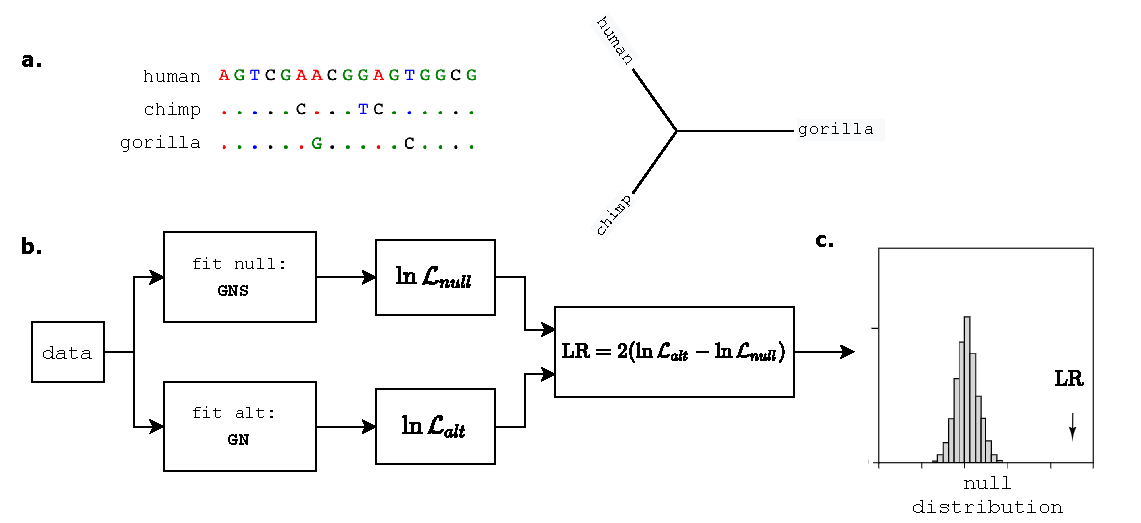
\includegraphics[width=\textwidth]{figures/diagrams/LRT.pdf}
\caption{\textbf{Likelihood Ratio Test.} \textbf{a}, The data: an alignment of orthologous sequences for human, chimp and gorilla, and a phylogenetic tree indicating the relationship between taxa. \textbf{b}, A LRT comparing substitution models, GNS is the null and GN is the alternate. The log-likelihood ($\ln\mathcal{L}$) for each model is obtained via fitting. The likelihood ratio (LR), is the ratio of the $\ln\mathcal{L}$ of the two models. \textbf{c}, the LR statistic is compared to the null distribution. In this case the statistic exceeds the distribution of values we would expect if the null was true, we would thus conclude that process is described significantly better with the alternate (GN) process.}
\label{fig:lrt}
\end{figure}

\section{Defining Novel Statistical Measures}
\label{Novel Statistical}

\subsection{Test of Existence}
\label{Test of Existence}

To test for the existence of mutation disequilibrium I have formulated an LRT, denoted the Test of Existence (TOE). The two models fundamental to this test are GN and GNS. Their point of difference is that the parameters of a GNS rate matrix must satisfy $\pi\mathbf{Q}=0$, i.e., the process is constrained to be stationary (and thus in equilibrium). Consider an LRT in which GNS is the null and GN is the alternate. If we reject the null, we have some evidence that the sequences are more likely to have been generated by a process that is not yet stationary, as this is the only component unique to the alternate.

An LRT as described above is too naive for my objective to test for equilibrium in a single lineage. For a GN model to be \gls{identifiable} requires an alignment of at least three sequences \citep{Chang1996FullConsistency}. Consequently, a significant result for such an LRT will not reveal which of the taxa is causing the rejection of the null. To test for disequilibrium in a single \gls{edge} I model a continuous-time process on the edge of interest (herein the foreground edge) and discrete-time processes for the other edges (herein the background edges) \citep{Verbyla2013TheSubstitution}. I expect the root of the tree to occur on one of the background edges, at which point the direction of time will swap. A discrete-time process is more general and can accommodate this potential confounder, as well as changes in mutagenesis on the background edges \citep{Verbyla2013TheSubstitution}. 

Using mixed discrete- and continuous-time Markov processes, I can test for the existence of disequilibrium on a single edge. For such an LRT, the foreground edge assumes GNS for the null, and GN for the alternate. Both hypotheses assume a Barry and Hartigan (BH) model for the background edges \citep{Barry1987StatisticalEvolution}. The TOE is an LRT between the following two hypotheses: \\ \textbf{Null}: the foreground evolved according to the \textbf{GNS}, the background according to BH. \\ \textbf{Alt}: the foreground evolved according to the \textbf{GN}, the background according to BH.\\ The modelling of the foreground edge, set apart by the assumption of stationarity, is the only point of difference between hypotheses. For this LRT, a rejection of the null means that the foreground edge was described significantly better with a non-stationary process. Such a result suggests disequilibrium precisely in the foreground edge. Herein all TOE model fits assume mixed discrete- and continuous-time Markov processes, and a BH process is always assumed for the background edges. For brevity, I will refer to a model by the process assumed on the foreground edge.

\subsection{$\nabla$}
\label{nabla}

I present a novel statistic $\nabla$, which is a measure of the speed of convergence of the substitution process to equilibrium. Consider a process operating on a single edge of a phylogenetic tree for time interval $t$, with $\pi_0$ the frequencies of nucleotides at the root and the rate matrix $Q$ on the edge. The nucleotide distribution at $t$ is $\pi(t) = \pi_{0} \cdot e^{Qt}$. For a stationary process, this simplifies to $\pi(t) = \pi_{0}$. Under weak assumptions, a non-stationary process will converge to a stationary process, for which $\pi$ remains unchanged over time. Thus, I can describe the speed of this convergence with the rate of change of $\pi(t)$. In other words, the derivative of $\pi$ with respect to $t$,
\begin{equation}
\label{eq:dpi/dt}
\frac{\partial \pi}{\partial t}(t) = \pi_{0} \cdot Q \cdot e^{Qt}.
\end{equation}

To describe the magnitude of a vector in a single value, it is natural to take its length. Accordingly, the $\nabla$ statistic is defined as follows,
\begin{equation}
\label{eq:len-dpi/dt}
\nabla = ||\frac{\partial \pi}{\partial t}(t)|| =|| \pi_{0} \cdot Q \cdot e^{Qt}||.
\end{equation}
$\nabla$ is the magnitude of the rate of change of $\pi(t)$. For a stationary process, for which by definition $\pi$ does not change over time, $\nabla = 0$. For a non-stationary process, as the process approaches equilibrium, $\nabla$ will asymptote to $0$. For a given non-stationary process that converges monotonically to equilibrium, $\nabla$ must increase the further one moves from equilibrium. The algorithm used to calculate $\nabla$ is presented in Algorithm \ref{alg:convergence}.

\begin{algorithm}[ht!]
\caption[Algorithm]{Calculating $\nabla$}
\label{alg:convergence}
\begin{minted}{python}
def convergence(pi_0, Q, t):

    pi_deriv = dot(pi_0, dot(Q, expm(Q * t)))
    conv = norm(pi_deriv)

    return conv
\end{minted}
\end{algorithm}


\subsection{$T_{50}$}
\label{T50}

A seemingly natural way to describe disequilibrium in a system is by its proximity to equilibrium. As previously stated, for a process in disequilibrium, as time goes to infinity, its nucleotide distribution will converge to $\pi_\infty$, its equilibrium distribution. This can be expressed mathematically as 
$$\pi_\infty = \lim_{t \to \infty}\pi \cdot e^{\mathbf{Q}t}.$$ 
This property manifests in other situations, for example, the decay of a radioactive element. In those fields the problem of quantification is solved by expressing in terms of an arbitrarily chosen metric, half-life, the time taken until half of the element's original mass is left. $T_{50}$ is defined equivalently. ${T_{50}}$ is a measure of the distance to halfway to $\pi_\infty$, measured in terms of the expected number of substitutions. The algorithm used to calculate $T_{50}$ is presented in Algorithm \ref{alg:t50}.

\begin{algorithm}[ht!]
\caption[Algorithm]{Calculating $T_{50}$}
\label{alg:t50}
\begin{minted}{python}
class T50:
    def __init__(self, Q, pi_0, func=jsm):
        """
        func
            a callback function that takes two probability vectors
            and returns a "distance". Defaults to Jensen-Shannon metric.
        """
        self.Q = Q
        self.pi_0 = pi_0
        self.pi_inf = self.get_stat_pi()
        self.dist_halfway = func(self.pi_0, self.pi_inf) / 2
        self.tau = 1
        self.dist_func = func

    def get_stat_pi(self):
        return get_stat_pi_via_brute(expm(self.Q), self.pi_0)

    def estimate_t50(self):
        ens_curr = expected_number_subs(self.pi_0, self.Q, 1)
        self.tau = minimise(
            self,
            xinit=self.tau,
            bounds=([1], [1e10]),
            local=True,
            show_progress=False,
            tolerance=1e-8,
        )
        ens_50 = expected_number_subs(self.pi_0, self.Q, self.tau)
        return ens_50 - ens_curr

    def distance_from_pi_zero(self, pi):
        return self.dist_func(self.pi_0, pi)

    def __call__(self, tau):
        pi_tau = dot(self.pi_0, expm(self.Q * tau))
        dist1 = self.dist_func(self.pi_0, pi_tau)
        dist2 = self.dist_func(pi_tau, self.pi_inf)
        return abs(dist1 - dist2) ** 2
\end{minted}
\end{algorithm}


\subsection{Tests of Equivalence of Process}
\label{Tests of Equivalence of Process}
To test for equivalence of the evolutionary process I have defined two LRTs. The question of equivalence applies to two comparisons: adjacent, for the comparison of linked physically adjacent genes in the same species; and temporal, for the comparison of one-to-one orthologs.

\subsubsection{Adjacent }

The adjacent Equivalence of Process test (aEOP) is between linked physically adjacent genes in the same species. For a single alignment of three taxa, a split continuous- and discrete-time model can be specified by the following set of parameters: $( \bm{Q}_{fg}, \bm{P}_{bg1}, \bm{P}_{bg2}, \pi_{0}, b ) $ where $\bm{Q}_{fg}$ is a continuous-time rate matrix describing the foreground edge,  $\bm{P}_{bg1}$ and $\bm{P}_{bg2}$ are discrete-time probability substitution matrices each describing one of the background edges, $\pi_{0}$ is the motif probabilities in the most recent common ancestor, and $b$ is the branch length corresponding to the foreground edge. 

For the adjacent Equivalence of Process test (aEOP) between two alignments aln\_1 and aln\_2, the null hypothesis constrains both alignments to have the same root motif probabilities and the same rate matrix on the foreground edge, i.e.,  \\
\textbf{Null:} $\bm{Q}_{fg}(\text{aln\_1}) = \bm{Q}_{fg}(\text{aln\_2})$,  $\pi_0(\text{aln\_1}) = \pi_0(\text{aln\_2})$. \\
\textbf{Alt} all parameters are independent between alignments. 

\subsubsection{Temporal }

The temporal Equivalence of Process test (tEOP) is between two edges of the same ortholog. In this case, there are two edges of interest, so the process is modelled with all edges as continuous time process. Such a model is specified by the following set of parameters: $( \bm{Q}_{fg1}, \bm{Q}_{fg2}, \bm{Q}_{bg}, \pi_{0}, b_{fg1}, b_{fg2}, b_{bg}) $, where $\bm{Q}_{fg1}$ and $\bm{Q}_{fg2}$ are continuous-time rate matrices each describing foreground edges,  $\bm{Q}_{bg}$ is a continuous-time rate matrix describing the background edge, $\pi_{0}$ is the motif probabilities in the most recent common ancestor, and $ b_{fg1}, b_{fg2}, b_{bg}$ is the branch length corresponding to the foreground edge. 

For the tEOP, the null hypothesis constrains both foreground edges to have the same rate matrix, i.e., \\
\textbf{Null:} $\bm{Q}_{fg1} = \bm{Q}_{fg2}$  \\ 
\textbf{Alt:} all parameters are independent between alignments. 

\subsection{Bootstrapping Procedure}

A $\chi^2$ distribution can be approximated as the null distribution only if asymptotic assumptions are shown to hold. In cases where asymptotic assumptions are shown not to hold, to get a robust estimate of the significance of an LRT statistic, parametric bootstraps can be used to determine the null distribution \citep{Goldman1993StatisticalSubstitution}. For a given alignment the bootstrap procedure is: 
(1) simulate 100 alignments of the same length as the observed alignment using the parameters of the null, 
(2) perform the same fit of the null and the alternate hypotheses to each synthetic alignment, determining the LR for each.  
This procedure provides what the distribution of LR values would look like if the null hypothesis was true. The estimated $p$-value is the proportion of the null distribution greater or equal to the LR of the observed alignment. 

In order to indicate the reliability of an estimate of a statistic, confidence intervals can be computed. The procedure is similar to bootstrapping, the difference is that simulations are done under the alternate hypothesis. The 2.5th and 97.5th percentiles of the simulated distribution indicate the boundaries of where we expect the parameter estimate to fall 95\% of the time. 

\section{Experimental Design}

To expose the behaviour of the methods under both the null and alternate hypotheses, I complemented the simulation studies with empirical analyses with prior predictions. Having defined my methods, it is only with both of these components that I can have confidence in their properties. I carefully constructed stationary simulated data sets reflecting what I consider to be edge cases, described below in Section \ref{Simulating under the null}. This allows me to establish the consistency of the statistics with theoretical expectations. I chose two empirical applications for which I have considerable confidence that the data is a natural occurrence of the alternate hypothesis. These are the loss of DNA methylation in \textit{D. melanogaster} and the translocation of \textit{Fxy} in \textit{M. musculus}. Using the behaviour of the methods in the previous steps as a benchmark, I then consider the evolution of the human genome. The experimental design is illustrated in Figure \ref{fig:experimental_design}. 

\begin{figure}[htbp]
\centering
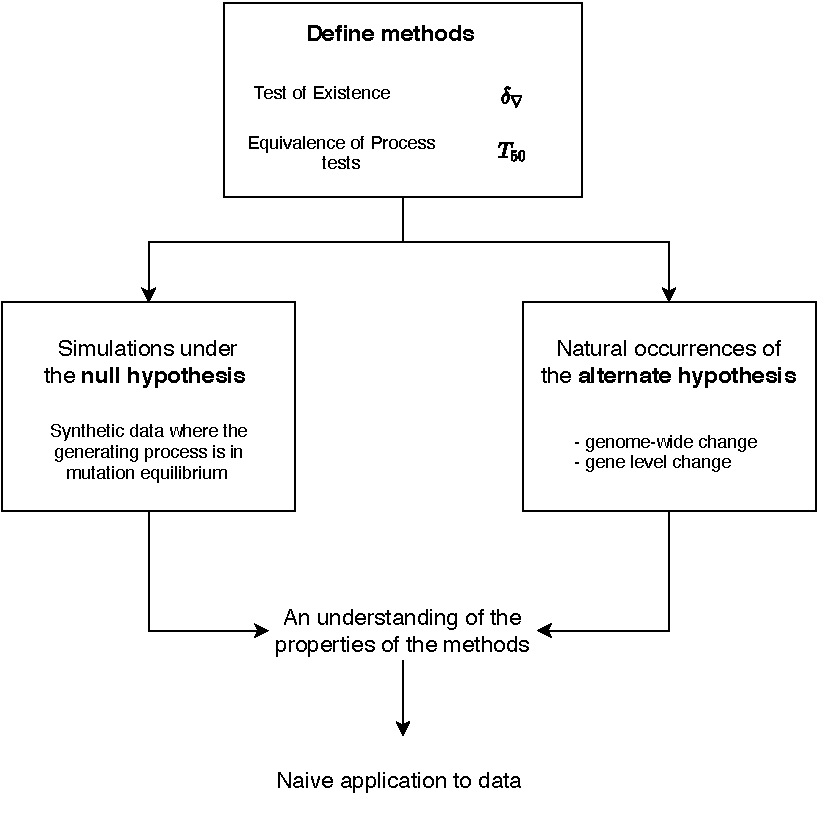
\includegraphics[width=\textwidth]{figures/diagrams/experimental_design.pdf}
\caption{Overview of experimental design process}
\label{fig:experimental_design}
\end{figure}

\subsection{Simulating under the null hypothesis}
\label{Simulating under the null}

One way to obtain data evolving under a GNS process (the null) is to exploit the fact that even a non-stationary process will converge to its stationary nucleotide distribution (herein $\pi_{\infty}$) as time goes to infinity. Essentially, I can obtain a GN model from real data, derive its corresponding $\pi_{\infty}$ and use those two things to define a stationary process. The process can be modified to model the background edges as discrete, and I can simulate alignments according to such a specification. This was my chosen simulation method as the resulting alignments are generated from parameters of real data. 

\subsubsection{Choosing Seed Alignments}

Using carefully diversified data allows for a thorough interrogation of my methods and how their properties may change when applied to different types of data. Natural data is a very large set of possible conditions. I can not possibly consider all conditions in simulated data. To overcome this, I identified what I considered to be the attributes of data that constitute edge cases, as they may define the boundaries of what I may encounter in nature. The potential confounders that I tried to address were the compositional skew, the magnitude of historic disequilibrium and the numerical stability of the process. These terms are defined below. Other natural confounders include the fact that the amount of data differs between different genomes and different sequence classes. I selected metrics to choose the seed alignments based on their ability to measure the considered confounders. 

An important measure I require is that of non-stationarity, which can manifest as a change in base composition over time. An indication of the degree of historical non-stationarity can be obtained from the difference in compositions between sequences in the same alignment. It is worth noting that studies of compositional data often require representation using Aitchison geometry. This representation allows for a consideration of the vulnerability of a composition to the sample it comes from. Although Aitchison geometry was initially considered, the composition of bases can also be considered as a probability distribution (i.e., $\pi = [\pi_T,\, \pi_G, \, \pi_C, \, \pi_A]$, such that $\pi_i$ where $i= \mathrm{T}, \mathrm{G}, \mathrm{C}, \mathrm{A}$ is the probability of observing the state $i$). In the case of comparing probability distributions, several measures can be used. My selected measure is the information-theoretic measure Jensen-Shannon Divergence (JSD). JSD measures the similarity between probability distributions. JSD was chosen as it can accommodate multiple distributions, allowing us to apply it to more than two sequences if needed. Additionally, it has an associated true metric, satisfying important mathematical properties (e.g., the triangle inequality). 

The base composition may affect the properties of my developed methods. Entropy is a fundamental quantity that indicates, in this case, the evenness of base composition. For example, $\pi =[1,\, 0,\, 0,\, 0]$  (a single nucleotide) has zero entropy whilst  $\pi =[0.25,\, 0.25,\, 0.25,\, 0.25]$ (equifrequent nucleotides) has the maximum possible entropy for 4 states. As a measure of compositional diversity, it captures an essential feature of the mode of evolution. Accordingly, the impact of compositions with different entropy is an important feature to consider in the process of method development.

 It is important to derive data from numerically stable processes. For a continuous-time process, the transition rate matrix $\mathrm{Q}$, specifies the instantaneous rates of exchanges between states. $\mathrm{Q}$ is foundational to a given substitution model. The eigendecomposition of $\mathrm{Q}$ is a representation of $\mathrm{Q}$ in terms of its eigenvalues and eigenvectors. Eigendecomposition is fundamental to many methods that I am using and developing. The condition number of a matrix is an indication of the suitability of the matrix to decomposition \citep{Schranz2008PathologicalPathogens}. Thus, I will use the $\mathrm{Q}$ matrix condition number to approximate the numerical stability of a process, so I am able to choose more numerically `stable' processes to generate data from.

Based on the above, I selected four microbial alignments to generate synthetic data sets and refer to these as seed alignments. As previously stated, I expect that JSD, entropy, and condition number may affect the numerical and or statistical properties of the developed methods. To derive data from numerically stable processes, all seed alignments were chosen from a subset of alignments where the condition number was low ($<2$). To capture the effect of historical disequilibrium (measured by JSD) and compositional skew (measured by entropy), the seed alignments represent the permutations of those extremes. These are: high JSD, low entropy; high JSD, high entropy; low JSD, low entropy; low JSD, high entropy. The ingroup taxa with the highest JSD with the outgroup was selected as the foreground edge. The attributes of each seed alignment are included in Table \ref{seed_alns} 

\begin{table}[htbp]
\centering
\small
\begin{tabularx}{\textwidth}{ 
  | >{\centering\arraybackslash}X
  | >{\centering\arraybackslash}X 
  | >{\centering\arraybackslash}X 
  | >{\centering\arraybackslash}X  
  | >{\centering\arraybackslash}X | }
\hline  
\textbf{Attributes} & \textbf{GreenGenes IDs} & \textbf{JSD} & \textbf{Entropy} & \textbf{Condition Number} \\
\hline 
\textbf{ High JSD, Low Entropy} & \textbf{573911}, 200580, 114946,  & 0.013269 & 1.562336 & 1.966567  \\
\hline
\textbf{ Low JSD, \hbox{Low Entropy}} & \textbf{73021}, 758, 443154 & 0.004523 & 1.66526 & 1.953336 \\
\hline
\textbf{High JSD, \hbox{High Entropy}} & \textbf{332182}, 17210, 197113 & 0.014152 & 1.785256 & 1.732004  \\ 
\hline
\textbf{Low JSD, \hbox{High Entropy}} & \textbf{206396}, 198257, 13724 & 0.002512 & 1.960842 & 1.407331 \\ 
\hline 
\end{tabularx}
\caption{\textbf{Attributes of seed alignments used for simulation}. The table shows the GreenGenes ID for all taxa in the species triple, JSD, entropy, and condition number. The ID of the edge modelled as the foreground is shown in bold.}
\label{seed_alns}

\end{table}


\subsubsection{Generating Synthetic Alignments that are Stationary, but not Reversible}
I expect the properties of my methods to be affected by the number of substitution events that distinguish the sequences in an alignment. The mathematical proof that LRT statistics are $\chi^{2}$ distributed assumes infinite data, that is the alignment is infinitely long. Although it has been shown that a few hundred base pairs can be sufficient for the $\chi^{2}$ to be accurate, this length is ultimately dependent on the number of substitution events \citep{Ota2000AppropriateParameters}. I can increase the number of events in a simulated alignment by increasing the length of the alignment.

It is necessary to determine how my methods are affected by the length of the alignment. I have done this by simulating multiple data sets differing in alignment length for all four seeds. The lengths were chosen to be representative of the alignment lengths of my biological application. The shortest sequences I will be using are protein coding genes, for which the average length (using just the 3rd codon position) is about 300bp. For each of the four seeds, I generated data sets of alignment length 300bp, 3,000bp, and 30,000bp.   

Establishing the properties of the EOP tests requires modified simulated data sets. The null distribution of the adjacent equivalence of the process test was determined using pairs of synthetic alignments. The simulated data sets are collections of alignments that were generated from the same stationary process. By definition the generating process is equivalent, so any differences in model fits represent sampling error arising from finite data. Since the alignments were generated randomly, I constructed an artificial genome by arbitrarily ordering sequences and then performed a `sliding window' of size two to select pairs of alignments.

The null hypothesis for the temporal equivalence of process test is that the foreground edges are generated by the same process. This the not the case for the previously mentioned simulated data. To specify the null distribution I again used the four stationary seed alignments but defined the two foreground edges have the same generating parameters. Again, for each of the four seeds, I generated data sets of alignment length 300bp, 3,000bp, and 30,000bp.

Each simulation set consisted of 1,000 synthetic alignments generated from the same function, derived from the parameter estimates from one seed alignment. An overview of the simulation process is described in Figure \ref{fig:simulating_alns}.

\begin{figure}[!ht]
\centering
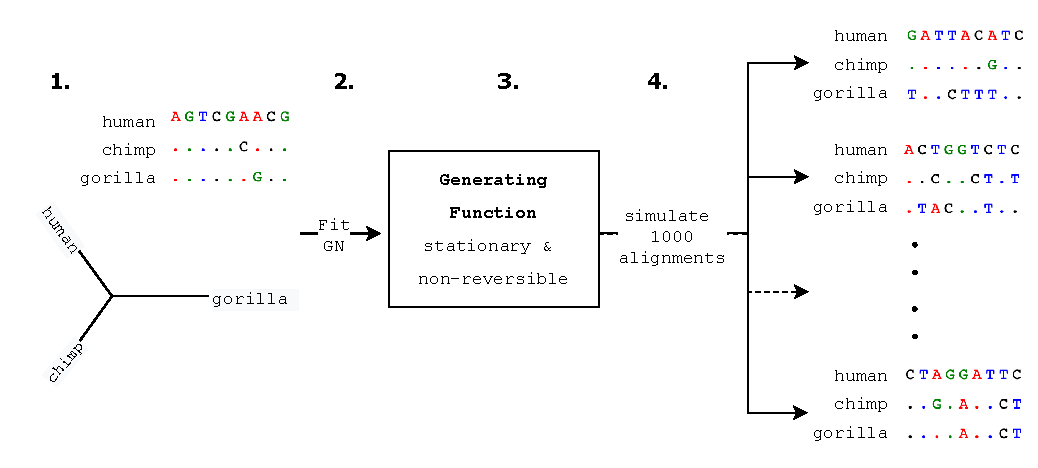
\includegraphics[width=\textwidth]{figures/diagrams/simulating_alns.pdf}
\caption{Creating synthetic data sets whose evolution was stationary but not reversible. \textbf{1,} select seed alignment, \textbf{2}, fit GN mixed model and extract model parameter estimates, \textbf{3}, define generating function using parameter estimates altered to be stationary, \textbf{4}, generate 1000 alignments of length $n$ and branch length scaled by $b$. For all 4 seeds this was performed for n = 300, 3000, 30000, and for each n, b = 1 and 3.}
\label{fig:simulating_alns}
\end{figure}

\subsubsection{Method of model fitting}

It is important to establish that the way in which the models are numerically optimised is reasonable. Additionally, the process of fitting a model to an alignment is the most time-consuming method routinely used in this project. I sought to identify the quickest possible method that yields a sufficiently maximised likelihood. For all synthetic data sets, I tested whether initialisation improved the model fitting process. The initialised method fit models in order of increasing generality (GTR, GNS, GN). Importantly, parameter estimates for each model were obtained from the previous model. The uninitialised method fit GNS and GN separately. The maximum likelihood estimates between uninitialised and initialised fits were compared for the models (e.g., uninitialised GN vs initialised GN). The time taken for each fitting process was recorded.  

\subsection{Empirical data with a prior expectation of disequilibrium}

I have chosen what I expect to be natural occurrences of the alternate hypotheses as positive empirical controls. In these cases I have a strong expectation of the existence of disequilibrium based on perturbations with respect to mutagenesis, leading to specific hypotheses about the expected form of mutation disequilibrium. The agreement between my predictions and results is an assessment of the ability of the developed methods to efficiently detect or measure mutation disequilibrium. 

\subsubsection{The loss of DNA methylation in \textit{D. melanogaster}}

$^5$mC, a well established mutagenic force, has been close to lost in \textit{D. melanogaster}. This radical change in the process acting upon the genome is expected to have induced a high level of mutation disequilibrium. Whether there are other causes of mutation disequilibrium in the \textit{D. melanogaster} genome is unknown. However, the level of mutation disequilibrium of its sister taxa, \textit{D. simulans}, is a useful approximation to the level of background disequilibrium. From this, I have a clear hypothesis, that the \textit{D. melanogaster} genome will exhibit higher levels of mutation disequilibrium at a greater magnitude than the \textit{D. simulans} genome. DNA methylation is a genome-wide phenomenon and therefore, I further predict that this relationship will be consistent on a genome-wide scale. 
 
\subsubsection{The translocation of \textit{Fxy} in \textit{M. musculus}}

The recent translocation of \textit{Fxy} in \textit{M. musculus} is a unique natural experiment. Meiotic recombination and its association with GC-biased gene conversion have been proposed to be a major force in the formation of isochores \citep{Montoya-Burgos2003RecombinationGenomes}. In which case, the translocation of \textit{Fxy} in \textit{M. musculus} has exposed half of the gene to a distinct environment. Not only is there a substantially higher rate of recombination, but the PAR is also recombining with the Y-linked section of \textit{Fxy}, exposed to the higher germ-line mutation rate of males \citep{Huttley2000HowMutagenesis}. The nature of this local rearrangement leads to specific hypotheses. I predict that the translocation in itself would lead to the existence of mutation disequilibrium in the entire gene. I further predict that there will be an elevated magnitude of disequilibrium in the region that has moved into the PAR, relative to the component of the gene that remains X-specific. 

\subsection{Naive application to The Great Apes}

The level of mutation disequilibrium in the Great Apes data set is unknown. It is, however, an extraordinarily well-curated genomic resource for which there is intronic and exonic sequence for the same genes. The application of methods to intronic data allows for a benchmark of the behaviour of methods in what is considered overwhelmingly selectively neutral data \citep{Graur2013OnENCODE}. 

\section{Algorithmic Implementation}

All methods described in this chapter, as well as all analyses presented in the results, were written using Python version 3.8. For all manipulation and analysis of biological sequence data, I used the develop branch of Cogent3 \citep{huttley_gavin_2021_4542532}, an open-source python library. The other major libraries used were NumPy 1.20.0 \citep{VanDerWalt2011TheComputation}, SciPy 1.6.0 \citep{SciPy2001}, Accupy 0.3.4 \citep{accupy} and Plotly 5.2.1 \citep{plotly}. All version control was managed by Git. To ensure reproducibility of the results, all variables of analyses, including all seeds used for random number generation, were logged using SciTrack 2020.6.5.

The code for all computation steps of the project is available in GitHub repositories that will be made public on submission of this work for publication. The scripts used for data sampling are included in KathData (https://github.com/GavinHuttley/KathData). All developed methods and other core library code are available in KathLibrary (https://github.com/GavinHuttley/KathLibrary). Script used to run analyses of data using the library code are available at KathAnalysis (https://github.com/GavinHuttley/KathAnalysis). The framework for algorithm testing used pytest. The code coverage is the degree of the source code which has been exercised by the test cases. The code coverage of the core library code was X\%. 

Analyses that required model fitting were performed on the National Computational Infrastructure's (NCI) supercomputer Gadi. Gadi uses a Linux operating system and analyses were run on multiple nodes comprising of 24-core Intel Xeon Scalable `Cascade Lake’ processors. All other analyses were performed on a MacBook Pro with four Intel i7 processors on which the  operating system was MacOS version 11.4. 